\begin{frame}{Experimentos - K-Fold}

\begin{itemize}
    \item K-Fold
    
      \begin{figure}
    \centering
    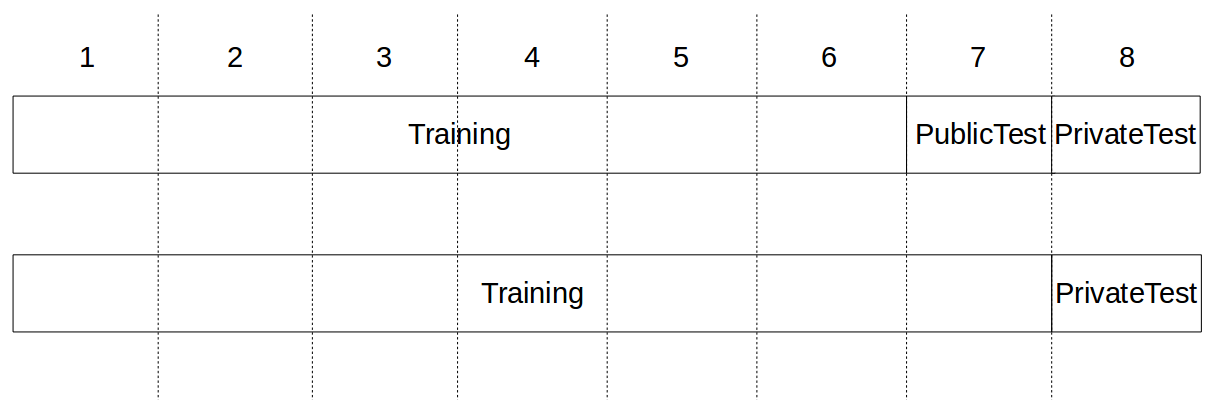
\includegraphics[width=1.0\linewidth]{img/evaluation.png}
    \caption{Divisão de partições do K-Fold.}
  \end{figure}
\end{itemize}

\end{frame}

\begin{frame}{Experimentos - Data augmentation}

    \begin{columns}
    \begin{column}{0.4\textwidth}
      \begin{itemize}
        \item Data augmentation
        \begin{itemize}
            \item Rotação
            \item Translação
            \item Escala
            \item Reflexão
        \end{itemize}
      \end{itemize}
    \end{column}
    
    \begin{column}{0.6\textwidth}
        \begin{figure}
    \centering
    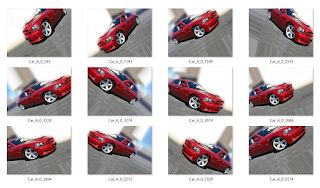
\includegraphics[width=1.0\linewidth]{img/data_augmentation.png}
    \caption{Data augmentation \cite{amaratunga_1970}.}
  \end{figure}
    \end{column}
    
\end{columns} 

\end{frame}

\begin{frame}{Experimentos - Medidas de desempenho}

    \begin{columns}
    \begin{column}{0.3\textwidth}
      \begin{itemize}
        \item Medidas
        \begin{itemize}
            \item F1-Score
            \item Acurácia
        \end{itemize}
      \end{itemize}
    \end{column}
    
    \begin{column}{0.7\textwidth}
        \begin{figure}
    \centering
    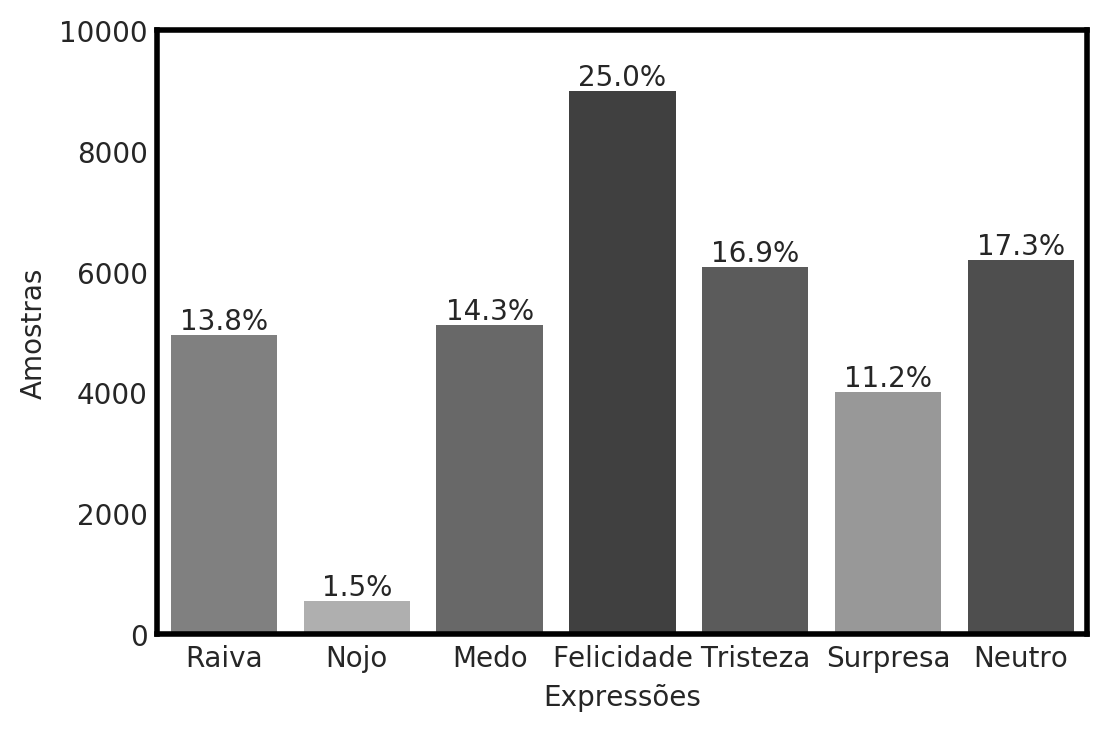
\includegraphics[width=0.9\linewidth]{img/expression_distribution.png}
    \caption{Distribuição de emoções na base de dados.}
  \end{figure}
    \end{column}
    
\end{columns} 

\end{frame}